\documentclass[zad,zawodnik,utf8]{sinol}

\title{Rowerzyści}
\id{row}
\author{Mateusz Radecki} % Autor zadania
\pagestyle{fancy}
\iomode{stdin}
\konkurs{XIV obóz informatyczny}
\etap{olimpijska}
\day{1}
\date{16.01.2017}
\RAM{256}
 
\begin{document}
\begin{tasktext}%

Przemek prowadzi hurtownię rowerów. Pewnego razu przyjechało do niego $n$ rowerzystów, pragnących kupić sobie rowery. Przypadkiem Przemek posiada dokładnie $n$ sztuk najnoszego $BikerUno2017$. Rowerzyści zapragnęli kupić je dla siebie, jednak nie wiedzą, jak powinni je między sobą rozdzielić.

Każdy szanujący się rowerzysta posiada swoją ulubioną liczbę. Ciąg $a_i$ oznacza właśnie ulubione liczby rowerzystów.

Każdy porządny rower posiada współczynnik $b_i$, zależny od wielu czynników, takich jak rodzaj opon, delikatność przerzutek, moc hamulca itp..

Rowerzysta jadący na rowerze posiada współczynnik fajności równy $a_i \cdot b_i$. Fajność grupy rowerzystów to suma po współczynnikach jej członków. Jako, że rowerzyści nie są zbyt dobrymi matematykami, to znają jedynie liczby od $0$ do $10^9+6$, dlatego zawsze gdy coś liczą, to wykonują obliczenia modulo $10^9+7$.

Przemek, jako znany cwaniak i dowcipniś, chciałby, aby fajność grupy rowerowej była jak najmniejsza, ponieważ to on chce być najfajniejszy na całym świecie. Chce więc tak przydzielić rowery rowerzystom, aby zminimalizować ich fajność (modulo $10^9+7$). Pomóż mu i znajdź takie przyporządkowanie.

Rowerzyści są jednak specyficzni. Każda ulubiona liczba rowerzysty jest losową liczbą z przedziału $[0, 10^9+6]$. To samo dotyczy współczynników rowerów typu $BikerUno2017$. Innymi słowy: każdy element ciągów $a_i$ i $b_i$ jest losowy. W szczególności dla każdego testu, na którym zostanie uruchomiony program, istnieją takie parametry $n$ i $seed$, że poniższy program po otrzymaniu tych argumentów generuje ten test.

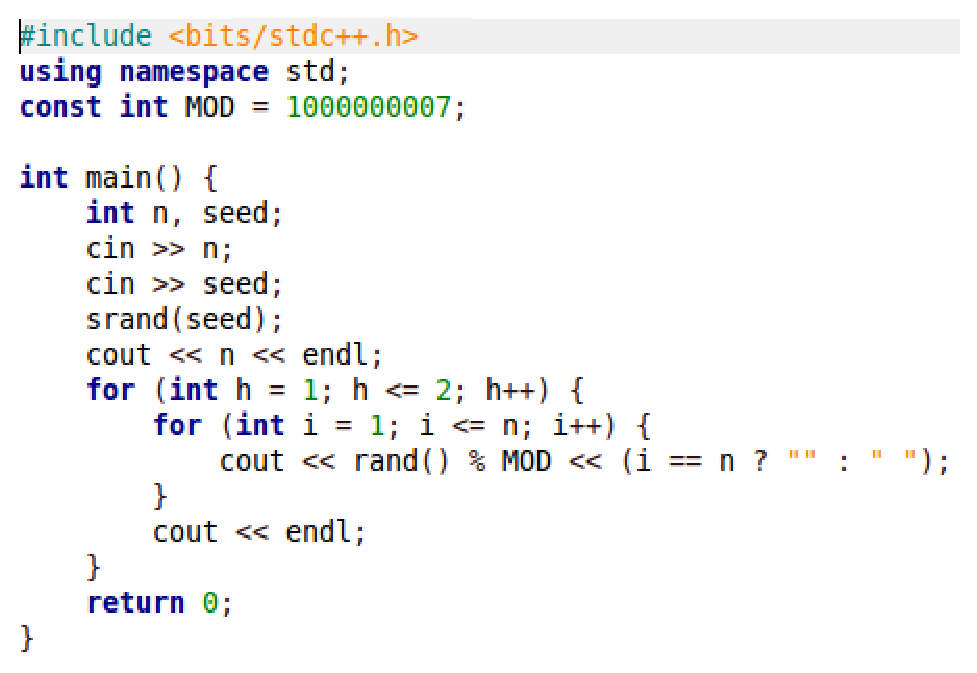
\includegraphics[height=7cm]{code.eps}

  \section{Wejście}
W pierwszym wierszu wejścia znajduje się liczba całkowita $n$ ($1 \leq n \leq 10^5$), oznaczająca liczbę rowerzystów i liczbę rowerów.

W kolejnym wierszu wejścia znajduje się $n$ liczb całkowitych $a_1, a_2, \cdots, a_n$ ($0 \leq a_i \leq 10^9+6$), oznaczające ulubione liczby rowerzystów.

W kolejnym wierszu wejścia znajduje się $n$ liczb całkowitych $b_1, b_2, \cdots, b_n$ ($0 \leq b_i \leq 10^9+6$), oznaczające współczynniki rowerów.

  \section{Wyjście}
W pierwszym wierszu wyjścia powinna znaleźć się jedna liczba całkowita, oznaczająca minimalną fajność grupy rowerzystów po przyporządkowaniu rowerów.
W drugim wierszu powinna znaleźć się permutacja $n$ liczb. Jeśli $i$-tą z tych liczb jest $x$, to znaczy, że $i$--temu rowerzyście chcemy przyporządkować $i$--ty rower.
  
\makecompactexample

\end{tasktext}
\end{document}
